\documentclass[a4paper,10pt]{article}
\usepackage[utf8]{inputenc}
\setcounter{tocdepth}{2} %Only show sections and subsections in toc.

\usepackage{colortbl}
\usepackage{siunitx} %Package for SI units
\sisetup{per-mode=fraction}

\usepackage{textcomp} %Vertically centered tilde (~)
\usepackage{amsmath}
\usepackage{graphicx}
\usepackage{standalone}

\usepackage[font={footnotesize}]{caption}
\usepackage[font={footnotesize}]{subcaption}

\usepackage[hidelinks]{hyperref}
%\hypersetup{
%    colorlinks = false,
%    linkbordercolor = {white},
%}


%\hypersetup{
 %   colorlinks,
 %   linkcolor={red!50!black},
 %   citecolor={blue!50!black},
 %   urlcolor={blue!80!black}
%}

\usepackage{float}
\usepackage[procnames]{listings}
\usepackage{epstopdf} %Convert EPS files to PDF format
\usepackage{pdfpages} %Utility to include pdf documents into the report, used to include datasheets in appendices.

\usepackage{tikz} 			%Utility to draw nice figures
\usetikzlibrary{shapes.geometric, arrows}
\usepackage{standalone}
\usepackage{circuitikz} 	%Utility to draw circuits in tikz

\usepackage[disable]{todonotes}
\usepackage{listings}
\usepackage{multirow}


\usepackage{url}
\renewcommand{\UrlFont}{\large\tt}

\usepackage{chngcntr} %Change the counters of objects. Used to make figure/table and equation counting specific to the section they are in.
\counterwithin{figure}{section}
\counterwithin{equation}{section}

%Make counter of listings specific to sections
\AtBeginDocument{%
  \counterwithin*{lstlisting}{section}
  \renewcommand{\thelstlisting}{%
    \ifnum\value{subsection}=0
      \thesection.\arabic{lstlisting}%
    \else
      \ifnum\value{subsubsection}=0
        \thesection.\arabic{lstlisting}%
      \else
        \thesection.\arabic{lstlisting}%
      \fi
    \fi
  }%
}

%\usepackage[inner=2cm,outer=4cm]{geometry}

\setlength{\parindent}{0pt}

\title{Electronics - 2. Semester Project}
\author{Thomas Søndergaard Christensen, Mikkel 
Skarup Jaedicke, Martin Brøchner Andersen, Catalin Ionut Ntemkas‎;}
\date{dd/mm/2016}


\begin{document}
%!TEX root = ../main.tex
\begin{titlepage}
%\newgeometry{left=3cm,right=3cm}
\begin{center}

\textsc{\LARGE University of Southern Denmark}\\[1.5cm]
\textsc{\Large MSc in Engineering - Electronics}\\
\textsc{\large 2. Semester Project}\\[0.5cm]

\vfill
\vspace{3cm}
\hrule ~\\[0.3cm]
{ \LARGE \bfseries Monitoring System for the SDU Go-Kart\\[0.4cm] }
\hrule ~\\[1.5cm]

\vfill

%\includegraphics[width=0.3\textwidth]{graphics/sdu_logo}
\vspace{7cm}
% Author and supervisor
\begin{minipage}[t]{.55\textwidth}
\begin{flushleft} \large
\textbf{Authors:}\\
230390 Martin Brøchner Andersen\\
151088 Catalin Ionut Ntemkas\\
030192 Mikkel Skaarup Jaedicke\\
100589 Thomas S. Christensen
\end{flushleft}
\end{minipage}
\begin{minipage}[t]{.44\textwidth}
\begin{flushright} \large
\textbf{Supervisor:} \\
Leon Bonde Larsen
\end{flushright}
\end{minipage}

\vspace{1cm}
Date: 19-12-2016

\vspace{1cm}

\end{center}
%\restoregeometry
\end{titlepage}
\newpage
\pagenumbering{Roman}
%!TEX root = ../main.tex
\section*{Preface}
\addcontentsline{toc}{section}{Preface}

\section*{Acknowledgment}
\addcontentsline{toc}{section}{Acknowledgment}
This project would not have been possible without the invaluable assistance and patience of our supervisor. 
A Tremendous thank you to Leon Bonde Larsen.
The process was simplified by Assistant Professor Kjeld Jensen from which the sensory equipment used in the report was supplied.
\thomas{Rewritten - needs a bit more?}
\martin{Who else should we thank? Viking Pizza?}
\mikkel{NEW URL}
\vspace{5cm}
\begin{center}
	\begin{minipage}[t]{.55\textwidth}\large
		\begin{center}
		Catalin Ionut Ntemkas\\
		\vspace{1cm}
		\hrule
		\vspace{0.5cm}
		Martin Brøchner Andersen\\
		\vspace{1cm}
		\hrule
		\vspace{0.5cm}
		Mikkel Skaarup Jaedicke\\
		\vspace{1cm}
		\hrule
		\vspace{0.5cm}
		Thomas Søndergaard Christensen
		\vspace{1cm}
		\hrule
		\end{center} 
	\end{minipage}
\end{center}

\vspace{1.2cm}
  \begin{center}
    \textsl{The report, source code, data, plotting script and simulations can be found at:}  
    \end{center}
    \vspace{-5pt}
    \begin{center}
	\renewcommand{\UrlFont}{\color{black}\normalsize\tt}
    \url{github.com/mikkeljae/SEM1PRO_ELECTRONICS}
   \end{center}
\newpage

\section*{Abstract}
\addcontentsline{toc}{section}{Abstract}
A go-kart has been supplied as a development platform for student projects at University of Southern Denmark.
In the interest of enabling more complex projects, a unified data collection system is necessary.
This is developed throughout this report. 
An analysis is done to determine the requirements of such a system.
It was found that a two-part network is suitable for this application.
The two parts are a CAN network and an ad-hoc WiFi network.
A custom protocol for use on CAN, GoCAN, is developed.
GoCAN supports up to 16 sensors from which data can be monitored on a remote monitoring station using the WiFi connection.
The system was only partially implemented since a connection between the CAN network and Linux was not achieved.
\thomas{Rewritten}
\newpage
\tableofcontents
\newpage
\listoftodos
%\listoftables
\clearpage
\newpage
\pagenumbering{arabic}
%!TEX root = ../main.tex
\section{System Description}
\label{sec:system_description}
This project is aimed at developing a backbone for data collection on the SDU go-kart.
As mentioned, the go-kart is intended as a development platform to be used by students on the master's programme in electronics on SDU.
Some projects may implement new sensory equipment while others may work on improving the inverter.
Common for all of them is that they require access to the data that their system is producing.
Providing a unified structure for gathering data from the go-kart will greatly ease the development on the platform, especially across different projects with different developers.
A system will be developed which provides a simple method for accessing data wirelessly on the go-kart while driving.
Live access of parameters while driving, realistically, requires some form of wireless communication between a monitoring system and the go-kart, see figure \ref{fig:simple}.

\begin{figure}[h]
 	\centering
    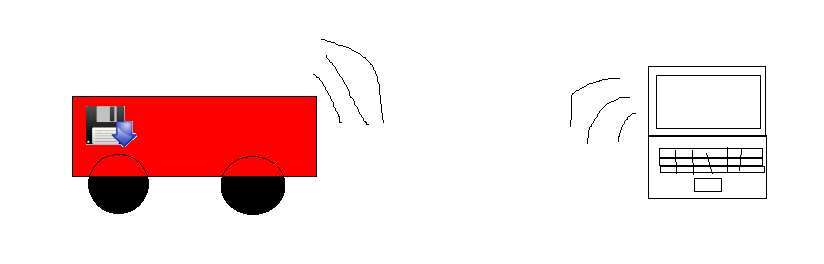
\includegraphics[width=0.6\textwidth]{graphics/go_kart_network_simple}
    \caption{SDU go-kart transferring data to a stationary computer wirelessly.}
    \label{fig:simple}
\end{figure}

While the system should be able to provide a live feed of the data being collected on the system, it should also log all data during a drive, with the possibility of transferring it later.
This will enable the user to do more advanced data analysis on the dataset than what can be achieved by monitoring the data.
In some cases, certain parameters may be irrelevant to the test being performed.
Transmitting these parameters should be avoidable by providing the possibility to start and stop data collection from specific data producers.

\begin{figure}[h]
 	\centering
    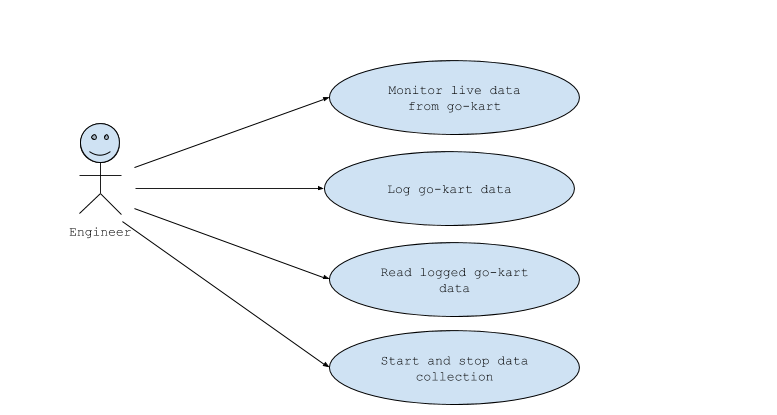
\includegraphics[width=1\textwidth]{graphics/use_cases}
    \caption{Use case diagram for the system.}
    \label{fig:usecases}
\end{figure}

As the goal of this system is to ease development on the go-kart, it should not only ease data collection, but also allow for simple addition of new sensors or other equipment.
Different projects may also have different requirements in terms of the presentation of data.
For this reason it should be possible to add a custom (G)UI of the projects design.
These requirements introduces a distinction between the actors expected to work with the system, the user and the developer.
The user will use the system to extract data from the system.
The developer will work on integrating new data producers into the system.
A use case narrative for each of the use cases is shown in appendix \ref{app:usecase}.
%!TEX root = ../main.tex

\section{Data Logging}
A feature will be data logging. 
Any data could be put into the log, although some signals can be logged at significantly higher rates than others
If all data is recorded at the fastest rate, this could present a storage problem.
This challenge will be analyzed here.
\subsection{Sample Rate}

Datalogging should be useful for working with an inverter as was the case on the first semester.
Likely it would be interesting to log the phase-current to the motor at high enough rate to accurately depict their sinusoidal short term average.
The ripple current or voltage at the motor terminals should be measured in the lab, as this requires a high sample rate, and more control than offered on the test track.
This data logging would be useful for recording current in the motor as the go kart is driving.
Additionally it would be relevant to record the encoder output, and possibly the DC voltage at the input of the inverter and the duty for each phase.
Only the currents are bound to change rapidly, and as such they determine the minimum acceptable sample rate.
By looking at the maximum frequency of the motor and the most extreme rate of change permissible by the armature inductance, it is possible to set a sample rate for the log file.\\

According to the manufacturer of the motor, the maximum rotational velocity is 5000 RPM.
With four pole pairs, this comes to a maximum sinusoidal frequency of 333 Hz. 
It is not necessary to record at a rate significantly larger than the Nyquist limit in order to adequately record the sinusoidal.
Simulations show, that by using Clark-Park transformation, interpolation and then the inverse Clarke-Park transformation, there is nearly no difference between a low sample rate of $1\si{\kilo\hertz}$, and a higher sample rate of $3.3\si{\kilo\hertz}$, as shown below.

\begin{figure}
	\centering
	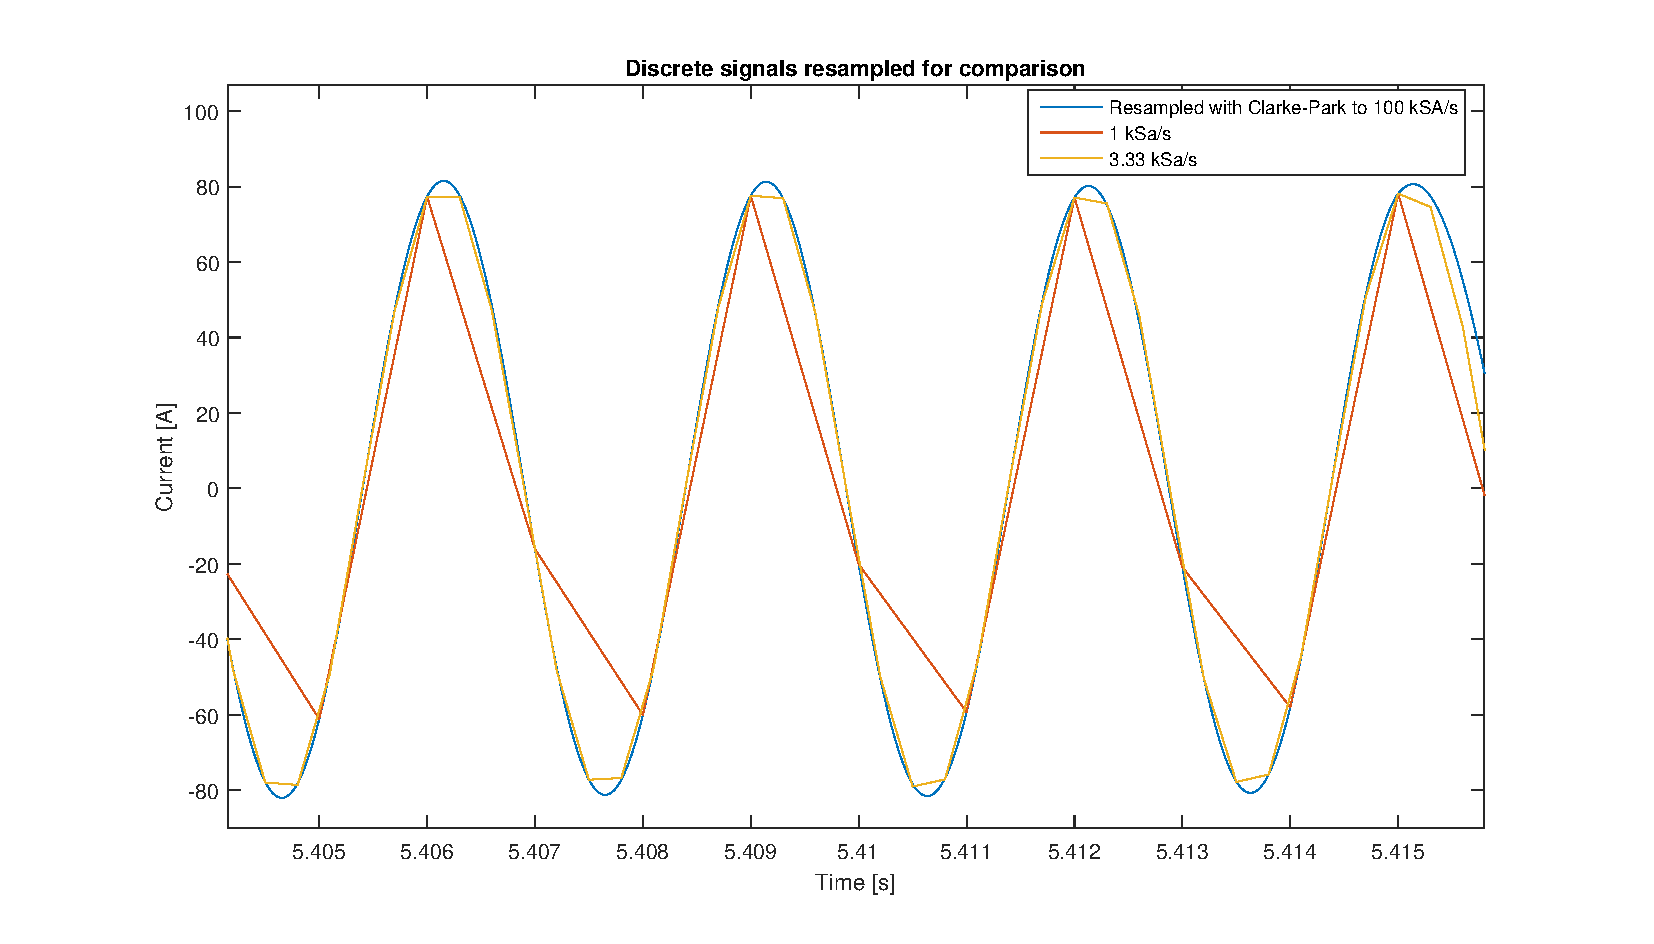
\includegraphics[width = 0.9\linewidth]{graphics/Clarke-park_resampled}	
	\caption{Comparison of data recorded at 1 kSa/s and 3.33 kSa/s, against 100 kSa/s resampled using Clarke-Park}
	\label{fig:Clarke-park_resampled}
\end{figure}

The resampled data from the 1 kSa/s and 3.3 kSa/s (orange and purple respectively on figure\ref{fig:Clarke-park_resampled}) are almost identical.
However, there is a small visible difference around the time 5.527 s, likely due to the limited precision of the encoder.
This also doesn't take into account any disturbance or noise, which could make it hard to reconstruct the signals with lower sample rates.\\

Additionally, the Matlab function, resample, produces nicely filtered vectors with smaller time steps, so it is possible to use a low sample rate for time invariant signals.\\
Another way to look at this is to calculate the maximum change in current from one sample to another.
This is determined by the inductance of the motor, which is $600 \si{\micro \henry}$ \todo[inline]{when one half bridge is high, and the two others are low, it's one armature inductance of 400 uH in series with two parallel armature inductances}, and the maximum voltage across it, which is $V_{BAT}=52.8 \si{\volt}$. 
At a sample rate of 3.33 kSa/s, this results in a theoretical maximum step of $264\si{\ampere}$.
A sample rate lower than this, would make it hard to properly record such sudden steps.

\subsection{Data Type}
When the sample rate is known, it is possible to get an estimate of how much storage space would be needed. 
It would be easiest, and most useful, to record using simple comma separated files, but these tend to take up more space than necessary.
The analog input to the Zybo are 12 bit, which means, that full precision of these would be possible with 4 digits, and often a decimal point and potentially a negative sign.
Including the horizontal separator, this comes to 6.5 bytes per point.\\

An example of recording could include time, two currents, a voltage and the encoder output, as displayed below
\begin{lstlisting}
Time	Ia	Ib	V	Encoder
1.0000	052.3	-278.1	52.56	16
1.0003	057.7	-280.4	52.54	17
\end{lstlisting}
That brings each line length to 32 bytes (8 bytes for time, 5.5 for the three analog, 3 bytes for encoder, 5 for separators).
At a sample rate of 3.33 kSa/s, this comes to 6.1MB per minute. 
With the current SD cards having 4 GB of free un-partitioned space, this gives up to 11 hours of recording time.\\

Alternately, it is possible to invent a file structure, that allows several arrays of with different data types.
By storing numbers in binary files instead of text, it is possible to reduce the space requirements to a third (2 bytes per analog, 4 bytes per timestamp (allowing up to 49 days of ms), and 1 byte for encoder).
This however will reduce the readability greatly, and include the workload, as one will need to write code both for encoding and decoding the file. \\

Since this is out of the scope of this project, and the sample rate isn't larger than it is, logging in standard ASCII will suffice.
Likely, different sample rates will be recorded to different log files
%!TEX root = ../main.tex
\todo{Each sentence should be on a new line. That way git more easily merges documents.}
\section{On-vehicle Local Network}

\subsection{Topology}

There are various network topologies that can be used to setup the required node network for this project.
These include the ring, bus, mesh ,star and tree topology.
Before we specify which one is suitable, a brief description of the purpose and functionality of our network as well as an overview of their advantages and disadvantages are needed. 

\subsubsection{Purpose of the Network}
\todo{Add the abbreviation ov = on-vehicle somewhere somehow}
The purpose of this network is to accommodate multiple nodes, such as sensors sub-networks and in general data-producers.
These need to be able to communicate with the main on-vehicle computer as well as among them.
The reasons for this is that the ov-computer is responsible for transmitting and receiving data from the stationary computer and other nodes may require data from other nodes to cooperate for a task.
Also, the ov-computer, apart from communicating, will also handle processing that the rest of the nodes are not able to. 
\\\\
The communication between the various nodes does not require a central hub.
Two nodes may need to communicate with one another without the control and the extra processing time of a centralized topology.
Furthermore, in the case that one fails, the network as a whole should still be operative.
Lastly, since it is a multi-node network and it may require more nodes in the future, a certain level of scalability is also required.

\subsubsection{Different Topologies}
\begin{itemize}
\item \textbf{Bus:} This is the simplest and cheapest topology.
All nodes communicate through a central bus and it is scalable with the addition of extra nodes on the two ends of the cable.
The central bus introduces the risk of complete network failure in case of the bus failure and the decrease in performance in case of many nodes or heavy traffic.
\item \textbf{Ring:} All the nodes in this type of network form a ring, where each node is connected to its two neighbors.
It has the advantages of the bus network as well and it shows better performance, even under heavy load.
A centralized control is not required for this type and in case of a node failure, the ring breaks and it can continue to function as a bus network.
It is scalable, but to a less extent than the bus.
\item \textbf{Mesh:} In this type, each node has direct connections to each other node present in the network.
That provides speed and reliability in case of node failures, but requires more hardware and processing power to manage the connections.
It is very robust but scalability is certainly not one of its features.
\item \textbf{Star:} The star topology is a centralized type of networking.
All nodes are connected to a central hub, handling all the communication between them.
It is fast, easy to implement and offers great reliability in case of node failures.
The major disadvantage is that if the hub fails, the entire network fails.
It can be scalable to a certain point, since the hub can be upgraded to handle more connections.
\item \textbf{Tree:} The last type, the tree is an extension of the bus and the star topologies combined.
It can be easily scalable, but that adds extra difficulty in its maintenance.
It also requires a lot of connections and in case the top (root) node fails, then all the network is down as well.
\item \textbf{Hybrid:} The last type is the hybrid one, where depending on the needs and purpose of the network, two or more topologies can be combined to achieve the best balance between their advantages and disadvantages.
\end{itemize}

\subsubsection{Suitable Topology}
For our networking purpose, the mesh type is not suitable, since it adds extra hardware requirements such as processing power and many redundant connections.
A node may be a simple sensor with a small microprocessor and hence, connecting it to such a network is not feasible.
In our system, a small embedded board computer will be the ov-computer which requires to maintain its connection with the network even in case of failures and also possibly the central hub in centralized topologies that such as the star and the tree.
Thus, these two topologies are not suited, since in case of its failure, the whole network fails.
Scalability is also a requirement for the future connection of nodes.
Although the majority of the types provide a level of scalability, the addition of extra nodes always decrease the overall performance of any network.
Hence, a topology that balances the decrease in performance against the network's expansion is best suited for the project.\\\\
The approach that fits the requirements is implementing a bus network, where each node may be a subnetwork of a different type depending on the needs, making it into a hybrid network having a bus topology as its basis.
This type provides a good balance of reliability, scalability, hardware requirements and communication speed in comparison to the others.

\subsection{Networking technology}

\subsubsection{Existing Technologies}
Different networking technologies exist in use today, such as Ethernet, CANbus, CANopen and Powerlink, among others.
CANbus is widely used in the automotive industry with data rates up to 1Mbit/s for small networks lengths, but the classic Ethernet and Powerlink support data rates of at least 10Mbit/s.
Furthermore, Powerlink is suitable for transmission of time-critical data and timing-synchronization of the nodes and CANopen networks are very robust and reliable.
\subsubsection{Choosing a Technology}
The two choices that were considered for the scope of this project were Powerlink and CANopen.
The first one can be implemented using openPowerlink at a software level and utilizing PmodNIC100 modules provided by the university.
On the other hand, CANopen can be implemented using CANopenSocket\footnote{https://github.com/CANopenNode/CANopenSocket}, an open source git project built on CANopenNode.
This library is easily implemented in Linux and can use various hardware, one of them being a USB to CAN interface board named USBtin\footnote{http://www.fischl.de/usbtin/}.
Another available module to use is the CANbus tranceiver breakout board from Copperhill which can be used by an IP core at a VHDL level that is available from Vivado IDE, greatly increasing the performance of such a network.
Since CANbus is a technology widely used in the automotive industry, it is our first choice for developing our system.

%Although for the purpose of this project Ethernet suffices, Powerlink adds a level for critical timing synchronization, a feature certainly needed for nodes that need to communicate and to react fast to a situation such as braking or to log data on a very small and specific time interval. Since the Zybo will be used possibly using PmodNIC100 modules as they are provided by the university, the openPowerlink protocol can be implemented in software utilizing as hardware the existing Ethernet ports provided by the modules. CAN-bus is also an option to implement with for example the CAN-bus tranceiver breakout board from Copperhill, and since it is a technology widely used in the automotive industry.
%link to CAN tranceiver: http://copperhilltech.com/can-bus-mini-breakout-board/
\begin{figure}
\caption{Use cases for the on-vehicle computer.}
\includegraphics[scale=0.7]{graphics/UML_UseCases_Zybo}
\end{figure}

\begin{table}[]
\centering
\caption{My caption}
\label{my-label}
\begin{tabular}{ll}
\multicolumn{1}{r}{\begin{tabular}[c]{@{}r@{}}Use case:\\ Actors:\\ Purpose:\\ Overview:\\ Type:\\ Preconditions:\\ Postconditions:\\ Special requirements:\end{tabular}} & \begin{tabular}[c]{@{}l@{}}Monitor live data from go-kart\\ Engi\end{tabular} \\
\multicolumn{1}{c}{Actor action}                                                                                                                                          & \multicolumn{1}{c}{System response}                                           \\
\begin{tabular}[c]{@{}l@{}}1.\\ 2.\end{tabular}                                                                                                                           &                                                                               \\
\multicolumn{2}{l}{Alternative flow of events}                                                                                                                                                                                                            \\
\multicolumn{2}{l}{Line?:}                                                                                                                                                                                                                              
\end{tabular}
\end{table}

\todo{Put the section about the Zybo use cases somewhere after Mikkel finishes.}


\newpage
%!TEX root = ../main.tex
\begin{thebibliography}{11} %This number should be higher than the number of entries in the bibliography because reasons...
%	\bibitem{id}
%		Author(s) Last name, First name, Company/Organisation, Year. Full Title
	\bibitem{xcanps}
			https://github.com/Xilinx/embeddedsw/blob/master/XilinxProcessorIPLib/drivers/canps/examples/xcanps\_polled\_example.c
	\bibitem{formulastudent}
			University of Southern Denmark, 2014, http://www.sdu-vikings.dk/
	\bibitem{ath9k}
			Open source, June 2015, https://wireless.wiki.kernel.org/en/users/drivers/ath9k\_htc/devices
	\bibitem{boostchat}
			www.boost.org, Boost C++ Libraries, http://www.boost.org/doc/libs/1\_62\_0/doc/html/boost\_asio/examples/cpp11\_examples.html
	\bibitem{beej}
			Hall, Brian, June 2016, Beej's Guide to Network Programming - Using Internet Sockets.
	\bibitem{CAN_introduction}
			Corrigan, Steve, Texas Instruments, July 2008, Introduction to the Controller Area Network (CAN).
	\bibitem{3.3V_CAN}
			Blackman, Jason and Monroe, Scott, Texas Instruments, January 2013, Overview of 3.3V CAN (Controller Area Network) Transceivers.
	\bibitem{interfacenaming}
			Open source, Nov 2015, Predictable Network Interface Names (https://www.freedesktop.org/wiki/Software/systemd/PredictableNetworkInterfaceNames/)
	\bibitem{xillinux}
			Xillybus LTD, http://xillybus.com/xillinux
	\bibitem{Xilinx_wiki_amp}
			Xilinx wiki Asymmetric Multiprocessing, http://www.wiki.xilinx.com/Multi-OS+Support+(AMP+\%26+Hypervisor)
	\bibitem{Xilinx_wiki_Linux_CAN_driver}
			http://www.wiki.xilinx.com/Linux+CAN+driver
	\bibitem{CANopen_introduction}
			http://www.ni.com/white-paper/14162/en/
	\bibitem{Xilinx_AMP}
			John McDougall, February 14, 2013, XAPP1078 v1.0, Simple AMP Running Linux and Bare-Metal System on Both Zynq SoC Processors, https://www.xilinx.com/support/documentation/application\_notes/xapp1078-amp-linux-bare-metal.pdf
	\bibitem{CAN-Utils}
			CAN-Utils tool, https://github.com/linux-can/can-utils/blob/master/README.md
	\bibitem{vectornav}
			VectorNav, vn-100 library, http://www.vectornav.com/support/downloads
	\bibitem{bluetooth}
			Wikipedia, Bluetooth, https://en.wikipedia.org/wiki/Bluetooth
	\bibitem{wiki_wifi}
			Wikipedia, IEEE\_802.11 , https://en.wikipedia.org/wiki/IEEE\_802.11\#Protocol
\end{thebibliography}
\martin{Check cites, ensure that they adhere to the thing and such}
\newpage
\end{document}

